

\section{Energy markets}

%Energy markets have emerged steadily from the mid-eighties. 

An outline of a possible implementation of a competitive energy market is depicted in \cite{hogan1993competitive} which is still valid as of today in many respects. A competitive market captures the advantage of market participants being able to actively shaping the clearing price applicable to both producers and consumers in the market. 




\subsection{Characteristics of energy markets}

Two main models exist for the exchange and types of trading of energy prices in power markets which are bilateral trading and electricity pooling, also called loose pool and tight pool models \cite{onaiwu2009does,hogan1997reshaping,barroso2005classification,reston2012short}.

\subsubsection{Loose pool models}

In bilateral trading or loose pool models utility operators (producers) and energy consumers establish bilateral contracts to determine the terms and conditions applied for trading energy \cite{onaiwu2009does,kalverboer2001electricity}. Generators or producers may also buy electricity from other suppliers in case their own electricity generation does not fit current demand. The exact amount, price and time when tradings take place are negotiated on the contract. Since electricity demand may vary from the negotiated terms the resulting imbalances have to be taken care of by the system operator. 

\subsubsection{Tight pool models}

Electricity pooling in tight pool models provide a way for utility operators to offer a certain amount of energy at a set price. Each generator places a bid containing the quantity and expected price \cite{barroso2005classification}. In return consumers place bids on how much they are willing to pay for a given amount of energy. The intersection of the aggregated demand and supply curves defines the energy price for that hour. 

Still customers, brokers and aggregators have the choice to either establish long term contracts of electricity or rely on the short-term market \cite{hogan1997reshaping}.



%Google Search "`loose pool models"'

%See also paper "`Electricity Transmission Pricing and Technology"' and chapter "`Making bilateral competition work"'

%\url{https://books.google.at/books?id=ycLrCAAAQBAJ&pg=PA282&lpg=PA282&dq=Electricity+Transmission+Pricing+and+Technology&source=bl&ots=okH3qUKJwi&sig=MTrGTYJRV5_KmJP9mbdo6GexiPg&hl=de&sa=X&ved=0CDIQ6AEwAmoVChMI3ce_q_XmxgIVBD8UCh1ngQpT#v=onepage&q=Electricity\%20Transmission\%20Pricing\%20and\%20Technology&f=false}


\subsubsection{Day ahead vs real time markets}

Both day ahead and real time markets exist within the scope of a deregulated wholesale power market. As discussed above, electricity pooling is a flexible way of determining energy prices for a short period of time in the future \cite{hogan1997reshaping}. Prices are set based on current demand and supply and are fixed for a particular point in time. This price is then valid for all market participants during that time period. 

In day ahead markets bids are placed for each consecutive hour of the following day. Thus prices are determined on a very short timescale and may exhibit significant volatility. Prices may change substantially from one hour to the next, up to a factor of ten \cite{huisman2007hourly}. Therefore market operators need to apply profound risk management techniques to alleviate such price spikes. 
%it is hard to predict

The real time market on the other hand is used to compensate demand variations during the day which may result in additional changes in energy prices. 
Due to this characteristic the real time market prices exhibit an even greater volatility than those at the day-ahead market whereby the latter is generally used for reference. 

%TODO Explain difference of intraday - real time markets. Same? See \url{http://www.nordpoolspot.com/How-does-it-work/Intraday-market/}. 

% Another resource (intraday market): https://www.next-kraftwerke.de/wissen/strommarkt/intraday-handel

% EPEX Spot - Intraday

%Der Intraday-Handel dient primär dazu, Fehlmengen oder Überschüsse des eigenen Bilanzkreises durch kurzfristige, untertägige Handelsaktivitäten so gering wie möglich zu halten, um den Prognoseverpflichtungen des Bilanzkreisvertrages nachzukommen und etwaige Ausgleichsenergiekosten zu reduzieren. Mit Hinblick auf immer flexibler werdende Anlagen lässt sich der kurzfristige Handel aber auch dafür nutzen, um den Strom von Anlagen kurzfristig bedarfsgerecht – und somit möglichst gewinnbringend und systemstabilisierend – zu produzieren.
%
%Der Intraday-Handel ist insbesondere von Bedeutung, um unvorhersehbare Änderungen in Stromproduktion und -nachfrage über marktliche Mechanismen aufzufangen, bevor der Einsatz von Regelenergie notwendig wird. So kann beispielsweise ein Kraftwerksbetreiber, in dessen Kraftwerk kurzfristig ein Block ausfällt, bei anderen Marktpartnern den seinem Bilanzkreis nun fehlenden Strom einkaufen. Dem Intraday-Handel kommt daher auch in der Direktvermarktung von Erneuerbaren Energien eine Schlüsselrolle zu, etwa wenn kurzfristig angepasste Wetterprognosen ein ungeplantes Mehr oder Weniger an Stromproduktion aus Solar- oder Windkraftanlagen verheißen.

%TODO Compare real time (5 min?) data with hourly day ahead data (graph). Evaluate volatility and maybe also forecasting behavior (this better suits under forecasting menu). 

% Negative Prices

% See https://www.epexspot.com/en/company-info/basics_of_the_power_market/negative_prices


\subsection{Outline of selected energy markets}



\subsubsection{Nord Pool Spot}


The NordPoolSpot market is the most mature power market to date and has been the first energy market that was established in Europe [c]. 

The NordPoolSpot power market consists of four different markets. %(... relevant citations are found below)

% Definition Website

% See http://www.nordpoolspot.com/How-does-it-work/

% THE POWER MARKET, emerging european energy market



As discussed before some markets exhibit strong seasonalities, while others do not. Nord Pool Spot is an example of a power market with obvious seasonalities in the data which can be taken advantage of when creating forecasting models. 

Below two hourly time series from two locations within Nord Pool Spot are displayed that show significant seasonal behavior. 
See figures \ref{fig:hourly_prices_finland} and \ref{fig:hourly_prices_sweden}.

\begin{figure}[!h]
	\centering
		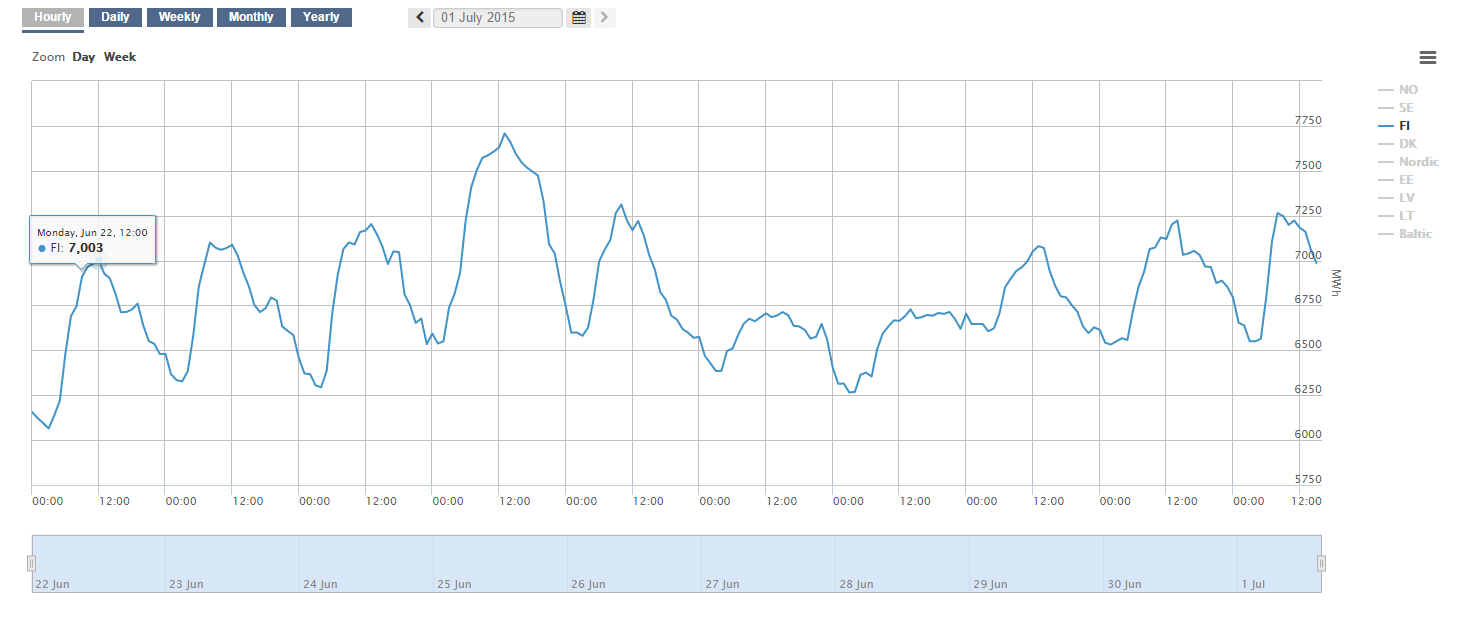
\includegraphics[width=1.00\textwidth]{figures/methodology/hourly_prices_finland.PNG}
	\caption{Finland hourly prices}
	\label{fig:hourly_prices_finland}
\end{figure}

\begin{figure}[!h]
	\centering
		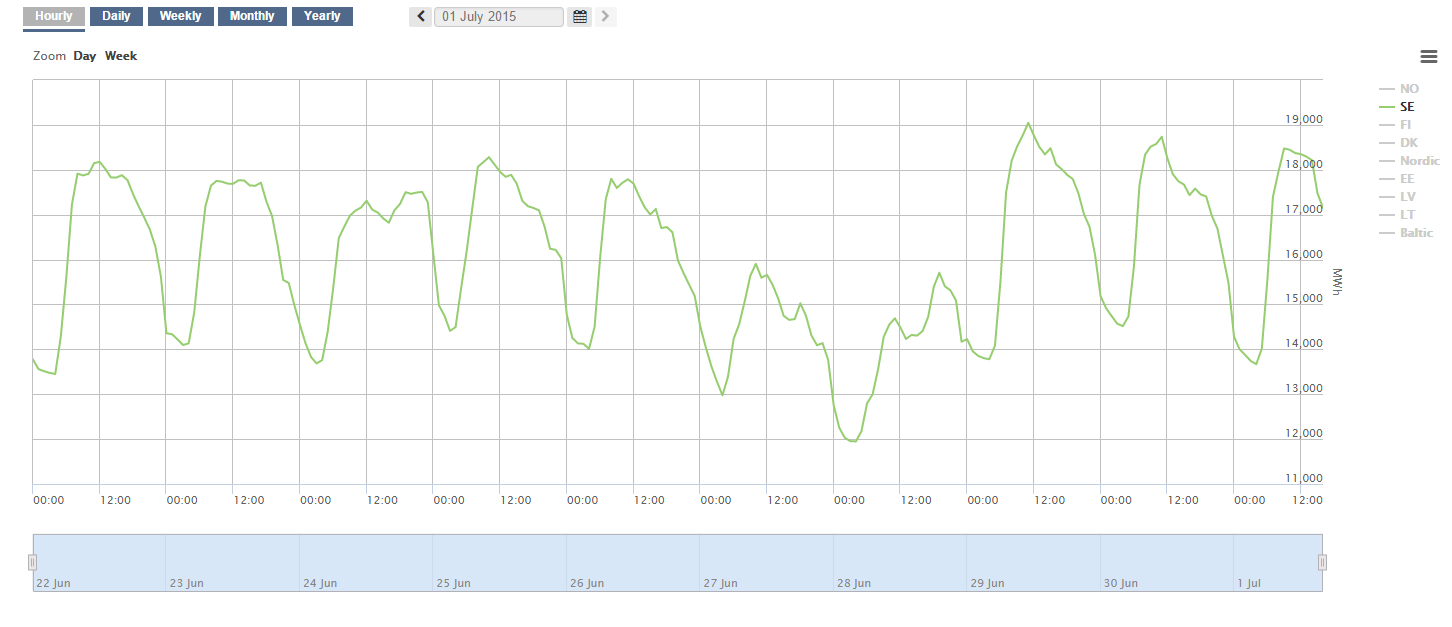
\includegraphics[width=1.00\textwidth]{figures/methodology/hourly_prices_sweden.PNG}
	\caption{Sweden hourly prices}
	\label{fig:hourly_prices_sweden}
\end{figure}




%
%
%[c BEGIN]
%
%\begin{itemize}[-]
%
%\item Financial market (Nasdaq OMX)
%Used for managing risks. Cash settled futures,
%forwards and options. Contracts can be made for
%up to six years. The system price is used as
%reference price.
%
%\item Day-ahead market (Nord Pool Spot)
%Day-ahead auction of power for delivery the next
%day. Nord Pool Spot calculates power prices
%based on supply and demand for every hour the
%following day.
%
%\item Intraday market (Nord Pool Spot)
%Continuous trading up to 30 minutes before
%delivery to adjust power production or
%consumption plans.
%
%\item Balancing market (TSOs)
%Operated by the respective transmission system
%operators. Final adjustments are made to ensure
%the correct frequency in the grid and security of
%supply
%
%\end{itemize}
%
%\emph{The future is Europe}
%
%The future of power trading lies in the
%creation of a single, integrated
%European market and an integrated
%platform.
%This will be the most advanced power
%market yet, offering efficiency in:
%
%\begin{itemize}
%\item Membership
%\item Management of collateral
%\item Cost
%\end{itemize}
%
%[c END] - Nord Pool Spot - Europe's leading power market \url{http://www.nordpoolspot.com/globalassets/download-center/annual-report/nord-pool-spot_europes-leading-power-markets.pdf}




%Nord Pool Spot - Day ahead market
%
%[c BEGIN]
%
%The day-ahead market, Elspot , is the main arena for trading power in the Nordic and Baltic region. Here, contracts are made between seller and buyer for the delivery of power the following day, the price is set and the trade is agreed.
%
%Today there are around 360 buyers and sellers (called members) on Elspot. Most of them trade every day, placing a total of around 2000 orders for power contracts on a daily basis.
%
%\emph{Driven by planning}
%
%Daily trading is driven by the members’ planning. A buyer, typically a utility, needs to assess how much energy (‘volume’) it will need to meet demand the following day, and how much it is willing to pay for this volume, hour by hour. The seller, for example the owner of a hydroelectric power plant, needs to decide how much he can deliver and at what price, hour by hour. These needs are reflected through orders entered by buyers and sellers into the Elspot trading system.
%
%\emph{Setting the price and closing the deal}
%
%12:00 CET is the deadline for submitting bids for power which will be delivered the following day. Elspot feeds the information into a specialist computer system which calculates the price, based on an advanced algorithm. Put simply, the price is set where the curves for sell price and buy price meet.
%
%\emph{Supply and demand}
%
%Hourly prices are typically announced to the market at 12:42 CET or later. Once the market prices have been calculated, trades are settled. From 00:00 CET the next day, power contracts are physically delivered (meaning that the power is provided to the buyer) hour for hour according to the contracts agreed.
%
%\emph{The cost of transmission constraints}
%
%While supply and demand are the key factors determining the hourly market prices, transmission capacity also plays a role. Bottlenecks can occur where power connections are linked to each other, if large volumes need to be transmitted to meet demand. To relieve this congestion, different area prices are introduced. In other words, when transmission capacity gets constrained, the price is raised to reduce demand in the areas affected.
%
%[c END] - Nord pool Spot Elspot Market \url{http://www.nordpoolspot.com/How-does-it-work/Day-ahead-market-Elspot-/}



%Nord Pool Spot - Intraday market
%
%[c BEGIN]
%
%Elbas  is an intraday market for trading power operated by Nord Pool Spot. Covering the Nordic and Baltic region as well as Germany and recently extended to include the UK, Elbas supplements Elspot and helps secure the necessary balance between supply and demand in the power market for Northern Europe.
%
%The majority of the volume handled by Nord Pool Spot is traded on the day-ahead market. For the most part, the balance between supply and demand is secured here. However, incidents may take place between the closing of Elspot at noon CET and delivery the next day. A nuclear power plant may stop operating in Sweden, or strong winds may cause higher power generation than planned at wind turbine plants in Germany. At Elbas, buyers and sellers can trade volumes close to real time to bring the market back in balance.
%
%Trading close to real time
%
%At 14:00 CET, capacities available for Elbas trading are published. Elbas is a continuous market, and trading takes place every day around the clock until one hour before delivery. Prices are set based on a first-come, first-served principle, where best prices come first – highest buy price and lowest sell price.
%
%Increasingly important
%
%The intraday market is becoming increasingly important as more wind power enters the grid. Wind power is unpredictable by nature, and imbalances between day-ahead contracts and produced volume often need to be offset. Elbas will play a key role in the development of intraday power trading in Europe. Future prospects indicate exponential growth, reaching 1.900 GW installed wind capacity worldwide in 2020 (Source: World Wind Energy Association). This type of market can be a key enabler to increase the share of renewable energy in the energy mix. 
%
%[c END] - Nord pool Spot Intraday Market \url{http://www.nordpoolspot.com/How-does-it-work/Intraday-market/}




\subsubsection{ISO New England}

The market of ISO New England offers day ahead as well as real time energy prices where day ahead prices are available at an hourly interval while (preliminary) real time prices are available both at hourly and five minute intervals\footnote{\url{http://www.iso-ne.com/}}. 

Current locational marginal prices (LMPs) can be downloaded from a base url\footnote{\url{http://www.iso-ne.com/static-transform/csv/histRpts/da-lmp/}} and a specialized suffix depending on the file and date (e.g.~WW\_DALMP\_ISO\_20150414.csv). In this case, files are provided in csv format for better machine processing. 

%Example: 
%\begin{verbatim}
	%H,"Date","Hour Ending","Location ID","Location Name","Location Type","Locational Marginal Price",
	%"Energy Component","Congestion Component","Marginal Loss Component"
	%D,"04/14/2015","02","4006",".Z.SEMASS","LOAD ZONE",14.82,14.85,0.01,-0.04
	%D,"04/14/2015","02","4007",".Z.WCMASS","LOAD ZONE",14.94,14.85,0.01,0.08
	%D,"04/14/2015","02","4008",".Z.NEMASSBOST","LOAD ZONE",14.84,14.85,0.01,-0.02
%\end{verbatim}

A summary of all data that is available is provided for day ahead as well as real time prices\footnote{\url{http://www.iso-ne.com/isoexpress/web/reports/pricing/-/tree/zone-info}}. It is described as ``zonal information'' on the website to emphasize the locational character of the prices. 


\subsubsection{EEX}

The European Energy Exchange (EEX) is a power market operating for the market area of France, Germany/Austria and Switzerland. Each of these regions exhibits a separate spot market where prices are traded for the respective country. 
The actual trading takes place on EPEX SPOT, an organisation that drives the integration of power markets in Europe where EEX is a part of. It consists of an intraday (real time) and day ahead market for trading during the day and for the next day, respectively. 

Several info products are available on the market for end-of-day data (EOD) that cover historical as well as current trading data from the spot and derivatives markets. 
Data is available on subscription for all of the above mentioned regions. Available data formats include csv, excel and xml files, provided on demand on a ftp server. 
Depending on the type of product and the time period available different fees apply and have to be paid in advance. 
Access is granted to a vast amount of historical energy price data for the derivatives as well as the spot market for energy and other commodities like natural gas and coal where both prices and trading volumes are included. 

Naming conventions designating the different areas of trading are defined as follows: 

\begin{itemize}

\item \emph{PHELIX} The Physical Electricity Index denotes the area of Germany and Austria

\item \emph{SWISSIX} The Swiss Index denotes the area of Switzerland

\item \emph{FRANCE} The index for France denotes the area of France

\item \emph{ELIX} The European Electricity Index defines prices valid for all of Europe (?)

\end{itemize}


\subsubsection{APG}

Austrian Power Grid\footnote{\url{http://www.apg.at/de/markt/strommarkt}}



\subsubsection{PJM}

See at \url{http://www.pjm.com/}. 


\subsubsection{OMIE - Spanish power market}

OMIE represents the wholesale energy market for the iberian region. \footnote{\url{http://www.omel.com/en/inicio}}

EDP (Energias de Portugal) is an energy company in cooperation with the wholesale electricity market for Spain, Portugal and is also responsible for delivery and transmission of energy to other countries. \footnote{\url{http://www.edp.pt/en/aedp/sectordeenergia/sistemaelectricoespanhol/Pages/SistElectES.aspx}}


\subsubsection{Brazilian power market}

The brazilian power market exhibits special conditions as it is heavily based on hydro power generation \cite{reston2012short}. In this market the tight pool model is applied where generation dispatch is centralized by an Independent System Operator (ISO). 



\subsection{Relevance of markets to cloud environments}


\subsection{[Terms and definitions]}

\subsubsection{Definition of 'Clearing Price'}

The following is a definition of clearing price from Investopedia\footnote{\url{http://www.investopedia.com/terms/c/clearingprice.asp}}. 

\begin{quote}
The specified monetary value assigned to a security or asset. This price is determined by the bid and ask process of buyers and sellers interested in trading the security.

In any exchange, sellers prefer to part with their assets for the highest price possible while investors interested in buying the same asset desire the lowest purchase price possible. At some point, a mutually agreeable price is reached between buyers and sellers. It is at this point that economists say the market has "cleared" and transactions take place. Thus, the clearing price of an asset is the price at which it was most recently traded.
\end{quote}



%google Search : "`tight pool models electricity"'
%
%Google Books "`Making Competition Work in Electricity"'
%\url{https://books.google.at/books?id=Pki4tu3P8iIC&pg=PA286\&lpg=PA286\&dq=tight+pool+models+electricity\&source=bl\&ots=drkU0A9H3C\&sig=m_J7JCkGjf5ydml2fdbFQB50ojE\&hl=de\&sa=X\&ved=0CCQQ6AEwAGoVChMIgoLZjffmxgIVTLYUCh3DEQBT#v=onepage\&q=tight\%20pool\%20models\%20electricity\&f=false}
%
%Also see Figure 3.2 in the book on page 43. 
%
%Chapter 4: Requirements for competition- Demand side

The clearing price is set at the intersection of the demand and supply curves, see Figure \ref{fig:market_demand_supply}



\begin{figure}[!h]
	\centering
		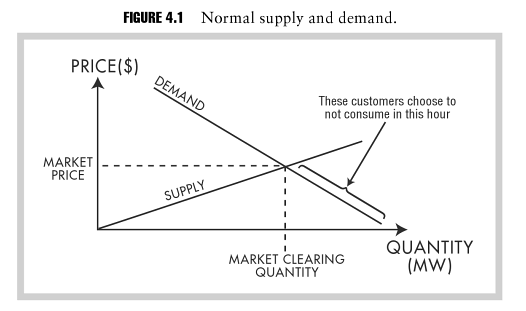
\includegraphics{figures/methodology/market_demand_supply.PNG}
	\caption{Demand Supply Chart}
	\label{fig:market_demand_supply}
\end{figure}



\subsubsection{Locational marginal price}

See definition by ISO-NE\footnote{\url{http://www.iso-ne.com/participate/support/faq/lmp}}. 

%TODO explain LMP (-> see ISO New England energy data, \textbf{smd hourly}!)

\subsubsection{System marginal price (SMP)}

A price type described by \cite{szkuta1999electricity}. 

\subsubsection{System Load}

%TODO

Some energy markets provide the total system load as measured by metering. It is used for day-ahead and long term forecasting purposes and in addition it serves as important indicator in reports. The system load for the ISO New England energy market is calculated by $System Load = generation - pumping + net\_interchange$


\subsubsection{Forward Capacity Market (FCM)} 

A forward capacity market is used to ensure having enough capacity for a specific amount of time into the future. A capacity commitment period (CCP) ensures that a certain amount of capacity will be available during that period. For example, the CCP at ISO-NE is set as one year ranging from June 1st until May 31st. 

The market has to ensure that the \emph{Installed Capacity Requirements (ICR)} for the corresponding region are met. These requirements are defined for each capacity commitment period and define the amount of capacity needed to meet estimated peak and reserve demands. Important measures to define the ICR are the local sourcing requirements (LSR) and maximum capacity limits (MCL) that define the constraints given by market participants. %(QUOTE)In addition the Hydro-Québec Interconnection Capability Credits (HQICCs), are a key input into the calculation of the ICR.

The actual procurement of resources for each capacity commitment period is determined by a \emph{Forward Capacity Auction (FCA)} which aims to meet the defined ICRs for the given period.
This auction is carried out three years ahead of the related CCP to ensure that enough resources will be available during that period. \emph{Reconfiguration Auctions (RA)} are then executed annually until the start of the CCP and continued monthly afterward. During an RA capacity resources may be amended to adapt to potential changes in capacity zones. 

At the FCM of ISO New England there is also the option of making a composite offer where different capacity resources may join their capacity offers (useful i.e.~in case of single season capacities) to result in a single resource offer at the market. 

%Capacity resources <-> energy suppliers/providers?

%See definition at the website of ISO NE\footnote{\url{http://www.iso-ne.com/markets-operations/markets/forward-capacity-market}}.

\subsubsection{Regulation market}

Definition by the ISO NE power market\footnote{\url{http://www.iso-ne.com/markets-operations/markets/regulation-market}}:

\begin{quote}
The Regulation Market is the mechanism for selecting and compensating market participants to provide regulation—the capability of specially equipped generators and other energy sources to increase or decrease output or consumption every four seconds. Participants allow their Automatic Generation Control (AGC) resources to be controlled by the ISO using automated signals to balance both second-by-second variations in demand and the system frequency, which must be kept constant. This market helps ensure that the ISO meets the North American Electric Reliability Corporation Real Power Balancing Control Performance Standard (BAL-001-0). Two regulation clearing prices are calculated: one for capacity and one for actual service mileage.
\end{quote}




\subsubsection{Two settlement system: Day ahead vs Balancing market}

A two settlement system has been defined for the PJM power market (PJM standing for Pennsylvania, Jersey, Maryland)\cite{lambert2001creating}. 

A two-settlement system in power markets is understood as a system comprising a day ahead as well as a real time (balancing) power market\cite{lambert2001creating}. 




\section{Forecasting}

\subsection{Forecasting of electricity prices}

Since the occurrence of competitive energy markets forecasting of energy prices has been vital to utility operators. 


\subsection{Outline of forecasting models}

%TODO
Discussion of suitable models for price time series from various energy markets. 


\subsubsection{Random walk}

A random walk model is best suited for series that exhibit major fluctuations on a short term and where no apparent trend can be recognized \cite{makridakisforecasting}(pg. 461). Thus this model can be described by an accumulation of a random error over time (equation \ref{eq:random_walk}). 

\begin{equation}
Y_t = \sum e_t
\label{eq:random_walk}
\end{equation}

$Y_t$ denotes the value of the time series at time point $t$ whereas $e_t$ is a timeseries of random errors where the errors exhibit no correlation and are normally distributed \cite{makridakisforecasting}(pg. 461). 

In \cite{makridakisforecasting}(pg. 464) it is stated that the behavior of economic and business series in particular can be characterized by a random walk model since they show so-called cycles or random fluctuations around a possible trend. 

As it is impossible to accurately predict upcoming values or cycles of a random walk model by definition one of the most suitable prediction models is the ``naive forecast'' where the forecasted value of the upcoming timestamp is set equal to the last observed value (equation \ref{eq:naive_forecast}).

\begin{equation}
\hat{Y}_{t+i} = Y_t
\label{eq:naive_forecast}
\end{equation}



\subsubsection{ARIMA models}

\emph{ARIMA model generation}

See Box-Jenkins Methodology. 


\subsubsection{Neural Network models}

An approach of using artificial neural networks (ANN) as a model to forecast short term electricity prices is presented in \cite{szkuta1999electricity}. 


\paragraph{Competition}

Neural network forecasting competition available from 2008\footnote{\url{http://www.neural-forecasting-competition.com/NN5/}}. 




\subsubsection{Forecasting benchmarks}






\subsection{Forecast accuracy measures}


\subsection{Model selection techniques}



\subsubsection{Autocorrelation}



The autocorrelation function determines the existence or non-existence of correlation between lagged variables within a time series. 

That is, the correlation between a point in the time series to another point in the same time series is calculated where the gap between the two points is fixed by the given lag. 

The autocorrelation is calculated as an autocorrelation coefficient in equation \ref{eq:autocorr_coeff}

\begin{equation}
R_h = \frac{C_h}{C_0}
\label{eq:autocorr_coeff}
\end{equation}


where $C_h$ denotes the autocovariance function and $C_0$ the variance function 
(see equations \ref{eq:autocov_func} and \ref{eq:variance_func}). 


\begin{equation}
C_h = \frac{1}{N} \sum\limits_{t=1}^{N-h} (Y_t - \bar{Y}) (Y_{t+h} - \bar{Y})
\label{eq:autocov_func}
\end{equation}


\begin{equation}
C_0 = \frac{1}{N} \sum\limits_{t=1}^{N} (Y_t - \bar{Y})^2
\label{eq:variance_func}
\end{equation}


Explanation: The autocovariance function determines the (average) covariance between variables with the given lag while the variance function determines the maximum (average) variance over all timestamps (t=1 to N). 


See \url{http://www.itl.nist.gov/div898/handbook/eda/section3/autocopl.htm}


\subsubsection{Box Cox transformation}

The Box Cox transformation is used to transform a series based on a non-normal distribution to a normal distribution. This is done via log and exponential transformations. 

See \url{http://www.isixsigma.com/tools-templates/normality/making-data-normal-using-box-cox-power-transformation/}



\subsection{Forecasting in cloud environments}



\section{Data center characteristics}

\subsection{Key indicators in data centers}

\subsection{Data management}

\subsection{Best practices in federated cloud environments}



\section{Cloud Simulation}

\subsection{Benefits and limitations}

\subsection{Simulation assumptions}

\subsection{Expected results}



\section{Summary}



